\documentclass[mstat,12pt]{unswthesis}

\usepackage{color}
\usepackage{fancyvrb}
\newcommand{\VerbBar}{|}
\newcommand{\VERB}{\Verb[commandchars=\\\{\}]}
\DefineVerbatimEnvironment{Highlighting}{Verbatim}{commandchars=\\\{\}}
% Add ',fontsize=\small' for more characters per line
\usepackage{framed}
\definecolor{shadecolor}{RGB}{248,248,248}
\newenvironment{Shaded}{\begin{snugshade}}{\end{snugshade}}
\newcommand{\AlertTok}[1]{\textcolor[rgb]{0.94,0.16,0.16}{#1}}
\newcommand{\AnnotationTok}[1]{\textcolor[rgb]{0.56,0.35,0.01}{\textbf{\textit{#1}}}}
\newcommand{\AttributeTok}[1]{\textcolor[rgb]{0.77,0.63,0.00}{#1}}
\newcommand{\BaseNTok}[1]{\textcolor[rgb]{0.00,0.00,0.81}{#1}}
\newcommand{\BuiltInTok}[1]{#1}
\newcommand{\CharTok}[1]{\textcolor[rgb]{0.31,0.60,0.02}{#1}}
\newcommand{\CommentTok}[1]{\textcolor[rgb]{0.56,0.35,0.01}{\textit{#1}}}
\newcommand{\CommentVarTok}[1]{\textcolor[rgb]{0.56,0.35,0.01}{\textbf{\textit{#1}}}}
\newcommand{\ConstantTok}[1]{\textcolor[rgb]{0.00,0.00,0.00}{#1}}
\newcommand{\ControlFlowTok}[1]{\textcolor[rgb]{0.13,0.29,0.53}{\textbf{#1}}}
\newcommand{\DataTypeTok}[1]{\textcolor[rgb]{0.13,0.29,0.53}{#1}}
\newcommand{\DecValTok}[1]{\textcolor[rgb]{0.00,0.00,0.81}{#1}}
\newcommand{\DocumentationTok}[1]{\textcolor[rgb]{0.56,0.35,0.01}{\textbf{\textit{#1}}}}
\newcommand{\ErrorTok}[1]{\textcolor[rgb]{0.64,0.00,0.00}{\textbf{#1}}}
\newcommand{\ExtensionTok}[1]{#1}
\newcommand{\FloatTok}[1]{\textcolor[rgb]{0.00,0.00,0.81}{#1}}
\newcommand{\FunctionTok}[1]{\textcolor[rgb]{0.00,0.00,0.00}{#1}}
\newcommand{\ImportTok}[1]{#1}
\newcommand{\InformationTok}[1]{\textcolor[rgb]{0.56,0.35,0.01}{\textbf{\textit{#1}}}}
\newcommand{\KeywordTok}[1]{\textcolor[rgb]{0.13,0.29,0.53}{\textbf{#1}}}
\newcommand{\NormalTok}[1]{#1}
\newcommand{\OperatorTok}[1]{\textcolor[rgb]{0.81,0.36,0.00}{\textbf{#1}}}
\newcommand{\OtherTok}[1]{\textcolor[rgb]{0.56,0.35,0.01}{#1}}
\newcommand{\PreprocessorTok}[1]{\textcolor[rgb]{0.56,0.35,0.01}{\textit{#1}}}
\newcommand{\RegionMarkerTok}[1]{#1}
\newcommand{\SpecialCharTok}[1]{\textcolor[rgb]{0.00,0.00,0.00}{#1}}
\newcommand{\SpecialStringTok}[1]{\textcolor[rgb]{0.31,0.60,0.02}{#1}}
\newcommand{\StringTok}[1]{\textcolor[rgb]{0.31,0.60,0.02}{#1}}
\newcommand{\VariableTok}[1]{\textcolor[rgb]{0.00,0.00,0.00}{#1}}
\newcommand{\VerbatimStringTok}[1]{\textcolor[rgb]{0.31,0.60,0.02}{#1}}
\newcommand{\WarningTok}[1]{\textcolor[rgb]{0.56,0.35,0.01}{\textbf{\textit{#1}}}}


%%%%%%%%%%%%%%%%%%%%%%%%%%%%%%%%%%%%%%%%%%%%%%%%%%%%%%%%%%%%%%%%%%
% 
% OK...Now we get to some actual input.  The first part sets up
% the title etc that will appear on the front page
%
%%%%%%%%%%%%%%%%%%%%%%%%%%%%%%%%%%%%%%%%%%%%%%%%%%%%%%%%%%%%%%%%%

\title{Projet réalisé par l'équipe 04\\[0.5cm]Rapport de groupe en
Sciences des Données 2 + Bases de données}

\authornameonly{MEDOM Michèle Marylyne/ NIYONKURU Berline
Cléria/ PALENFO Grace Sidiqa/ TAHARASTE Rayan }

\author{\Authornameonly}

\copyrightfalse
\figurespagefalse
\tablespagefalse

%%%%%%%%%%%%%%%%%%%%%%%%%%%%%%%%%%%%%%%%%%%%%%%%%%%%%%%%%%%%%%%%%
%
%  And now the document begins
%  The \beforepreface and \afterpreface commands puts the
%  contents page etc in
%
%%%%%%%%%%%%%%%%%%%%%%%%%%%%%%%%%%%%%%%%%%%%%%%%%%%%%%%%%%%%%%%%%%


%%%%%%%%%%%%%%%%%%%%%%%%%%%%%%%%%%%%%%%%%%%%%%%%%%%%%%%%%%%%%%%%%%%%%%%
%
%  A small sample UNSW Coursework Masters thesis file.
%  Any questions to Ian Doust i.doust@unsw.edu.au and/or Gery Geenens ggeenens@unsw.edu.au
%
%%%%%%%%%%%%%%%%%%%%%%%%%%%%%%%%%%%%%%%%%%%%%%%%%%%%%%%%%%%%%%%%%%%%%%%
%
%  The first part pulls in a UNSW Thesis class file.  This one is
%  slightly nonstandard and has been set up to do a couple of
%  things automatically
%
 
%%%%%%%%%%%%%%%%%
%% Precisely one of the next four lines should be uncommented.
%% Choose the one which matches your degree, uncomment it, and comment out the other two!
%\documentclass[mfin,12pt]{unswthesis}    %%  For Master of Financial Mathematics 
%\documentclass[mmath,12pt]{unswthesis}   %%  For Master of Mathematics
%\documentclass[mstat,12pt]{unswthesis}  %%  For Master of Statistics
%%%%%%%%%%%%%%%%%



\linespread{1}
\usepackage{amsfonts}
\usepackage{amssymb}
\usepackage{amsthm}
\usepackage{latexsym,amsmath}
\usepackage{graphicx}
\usepackage{afterpage}
\usepackage[colorlinks]{hyperref}
 \hypersetup{
     colorlinks=true,
     linkcolor=blue,
     filecolor=blue,
     citecolor= black,      
     urlcolor=cyan,
     }
\usepackage{textcomp}
\usepackage{longtable}
\usepackage{booktabs}
\usepackage{float}
\let\origfigure\figure
\let\endorigfigure\endfigure
\renewenvironment{figure}[1][2] {
    \expandafter\origfigure\expandafter[H]
} {
    \endorigfigure
}
\usepackage[T1]{fontenc}
\usepackage{ragged2e}
\def\tightlist{}

%%%%%%%%%%%%%%%%%%%%%%%%%%%%%%%%%%%%%%%%%%%%%%%%%%%%%%%%%%%%%%%%%
%
%  The following are some simple LaTeX macros to give some
%  commonly used letters in funny fonts. You may need more or less of
%  these
%
\newcommand{\R}{\mathbb{R}}
\newcommand{\Q}{\mathbb{Q}}
\newcommand{\C}{\mathbb{C}}
\newcommand{\N}{\mathbb{N}}
\newcommand{\F}{\mathbb{F}}
\newcommand{\PP}{\mathbb{P}}
\newcommand{\T}{\mathbb{T}}
\newcommand{\Z}{\mathbb{Z}}
\newcommand{\B}{\mathfrak{B}}
\newcommand{\BB}{\mathcal{B}}
\newcommand{\M}{\mathfrak{M}}
\newcommand{\X}{\mathfrak{X}}
\newcommand{\Y}{\mathfrak{Y}}
\newcommand{\CC}{\mathcal{C}}
\newcommand{\E}{\mathbb{E}}
\newcommand{\cP}{\mathcal{P}}
\newcommand{\cS}{\mathcal{S}}
\newcommand{\A}{\mathcal{A}}
\newcommand{\ZZ}{\mathcal{Z}}
%%%%%%%%%%%%%%%%%%%%%%%%%%%%%%%%%%%%%%%%%%%%%%%%%%%%%%%%%%%%%%%%%%%%%
%
% The following are much more esoteric commands that I have left in
% so that this file still processes. Use or delete as you see fit
%
\newcommand{\bv}[1]{\mbox{BV($#1$)}}
\newcommand{\comb}[2]{\left(\!\!\!\begin{array}{c}#1\\#2\end{array}\!\!\!\right)
}
\newcommand{\Lat}{{\rm Lat}}
\newcommand{\var}{\mathop{\rm var}}
\newcommand{\Pt}{{\mathcal P}}
\def\tr(#1){{\rm trace}(#1)}
\def\Exp(#1){{\mathbb E}(#1)}
\def\Exps(#1){{\mathbb E}\sparen(#1)}
\newcommand{\floor}[1]{\left\lfloor #1 \right\rfloor}
\newcommand{\ceil}[1]{\left\lceil #1 \right\rceil}
\newcommand{\hatt}[1]{\widehat #1}
\newcommand{\modeq}[3]{#1 \equiv #2 \,(\text{mod}\, #3)}
\newcommand{\rmod}{\,\mathrm{mod}\,}
\newcommand{\p}{\hphantom{+}}
\newcommand{\vect}[1]{\mbox{\boldmath $ #1 $}}
\newcommand{\reff}[2]{\ref{#1}.\ref{#2}}
\newcommand{\psum}[2]{\sum_{#1}^{#2}\!\!\!'\,\,}
\newcommand{\bin}[2]{\left( \begin{array}{@{}c@{}}
				#1 \\ #2
			\end{array}\right)	}
%
%  Macros - some of these are in plain TeX (gasp!)
%
\newcommand{\be}{($\beta$)}
\newcommand{\eqp}{\mathrel{{=}_p}}
\newcommand{\ltp}{\mathrel{{\prec}_p}}
\newcommand{\lep}{\mathrel{{\preceq}_p}}
\def\brack#1{\left \{ #1 \right \}}
\def\bul{$\bullet$\ }
\def\cl{{\rm cl}}
\let\del=\partial
\def\enditem{\par\smallskip\noindent}
\def\implies{\Rightarrow}
\def\inpr#1,#2{\t \hbox{\langle #1 , #2 \rangle} \t}
\def\ip<#1,#2>{\langle #1,#2 \rangle}
\def\lp{\ell^p}
\def\maxb#1{\max \brack{#1}}
\def\minb#1{\min \brack{#1}}
\def\mod#1{\left \vert #1 \right \vert}
\def\norm#1{\left \Vert #1 \right \Vert}
\def\paren(#1){\left( #1 \right)}
\def\qed{\hfill \hbox{$\Box$} \smallskip}
\def\sbrack#1{\Bigl \{ #1 \Bigr \} }
\def\ssbrack#1{ \{ #1 \} }
\def\smod#1{\Bigl \vert #1 \Bigr \vert}
\def\smmod#1{\bigl \vert #1 \bigr \vert}
\def\ssmod#1{\vert #1 \vert}
\def\sspmod#1{\vert\, #1 \, \vert}
\def\snorm#1{\Bigl \Vert #1 \Bigr \Vert}
\def\ssnorm#1{\Vert #1 \Vert}
\def\sparen(#1){\Bigl ( #1 \Bigr )}

\newcommand\blankpage{%
    \null
    \thispagestyle{empty}%
    \addtocounter{page}{-1}%
    \newpage}

%%%%%%%%%%%%%%%%%%%%%%%%%%%%%%%
%
% These environments allow you to get nice numbered headings
%  for your Theorems, Definitions etc.  
%
%  Environments
%
%%%%%%%%%%%%%%%%%%%%%%%%%%%%%%%

\newtheorem{theorem}{Theorem}[section]
\newtheorem{lemma}[theorem]{Lemma}
\newtheorem{proposition}[theorem]{Proposition}
\newtheorem{corollary}[theorem]{Corollary}
\newtheorem{conjecture}[theorem]{Conjecture}
\newtheorem{definition}[theorem]{Definition}
\newtheorem{example}[theorem]{Example}
\newtheorem{remark}[theorem]{Remark}
\newtheorem{question}[theorem]{Question}
\newtheorem{notation}[theorem]{Notation}
\numberwithin{equation}{section}

%%%%%%%%%%%%%%%%%%%%%%%%%%%%%%%%%%%%%%%%%%%%%%%%%%%%%%%%%%%%%%%%%%
%
%  If you've got some funny special words that LaTeX might not
% hyphenate properly, you can give it a helping hand:
%

\hyphenation{Mar-cin-kie-wicz Rade-macher}


\newlength{\cslhangindent}
\setlength{\cslhangindent}{1.5em}
\newlength{\csllabelwidth}
\setlength{\csllabelwidth}{3em}
\newenvironment{CSLReferences}[2] % #1 hanging-ident, #2 entry spacing
 {% don't indent paragraphs
  \setlength{\parindent}{0pt}
  % turn on hanging indent if param 1 is 1
  \ifodd #1 \everypar{\setlength{\hangindent}{\cslhangindent}}\ignorespaces\fi
  % set entry spacing
  \ifnum #2 > 0
  \setlength{\parskip}{#2\baselineskip}
  \fi
 }%
 {}
\usepackage{calc} % for \widthof, \maxof
\newcommand{\CSLBlock}[1]{#1\hfill\break}
\newcommand{\CSLLeftMargin}[1]{\parbox[t]{\maxof{\widthof{#1}}{\csllabelwidth}}{#1}}
\newcommand{\CSLRightInline}[1]{\parbox[t]{\linewidth}{#1}}
\newcommand{\CSLIndent}[1]{\hspace{\cslhangindent}#1}






\renewcommand{\contentsname}{Table des matières}

\renewcommand{\chaptername}{Chapitre}



\begin{document}

\beforepreface

%\afterpage{\blankpage}

% plagiarism

\prefacesection{Déclaration de non plagiat}

\vskip 2pc \noindent Nous déclarons que ce rapport est le fruit de notre seul travail, à part lorsque cela est indiqué  explicitement. 

\vskip 2pc  \noindent Nous acceptons que la personne évaluant ce rapport puisse, pour les besoins de cette évaluation:
\begin{itemize}
\item la reproduire et en fournir une copie à un autre membre de l'université; et/ou,
\item en communiquer une copie à un service en ligne de détection de plagiat (qui pourra en retenir une copie pour les besoins d'évaluation future).
\end{itemize}

\vskip 2pc \noindent Nous certifions que nous avons lu et compris les règles ci-dessus.\vspace{24pt}

\vskip 2pc \noindent En signant cette déclaration, nous acceptons ce qui précède.
\vskip 2pc \noindent
Signature: \rule{7cm}{0.25pt} \hfill Date: \rule{4cm}{0.25pt} \\[1cm]
Signature: \rule{7cm}{0.25pt} \hfill Date: \rule{4cm}{0.25pt} \\[1cm]
Signature: \rule{7cm}{0.25pt} \hfill Date: \rule{4cm}{0.25pt} \\[1cm]
Signature: \rule{7cm}{0.25pt} \hfill Date: \rule{4cm}{0.25pt} \\[1cm]
\vskip 1pc



%\afterpage{\blankpage}


\afterpreface





%%%%%%%%%%%%%%%%%%%%%%%%%%%%%%%%%%%%%%%%%%%%%%%%%%%%%%%%%%%%%%%%%%
%
% Now we can start on the first chapter
% Within chapters we have sections, subsections and so forth
%
%%%%%%%%%%%%%%%%%%%%%%%%%%%%%%%%%%%%%%%%%%%%%%%%%%%%%%%%%%%%%%%%%%



%%%%%%%%%%%%%%%%%%%%%%%%%%%%%%%%%%%%%

%\afterpage{\blankpage}


\hypertarget{pruxe9sentation-du-thuxe8me}{%
\chapter{Présentation du thème}\label{pruxe9sentation-du-thuxe8me}}

\medskip

\textbf{« Où rouler en sécurité » } tel est le thème que nous avons
choisi d'explorer. Pour aborder ce thème, il nous semble évident
d'identifier les circonstances les plus dangereuses sur la route afin
d'y être le plus en sécurité possible. Cela nous amène à nous poser
alors cette question :

\bigskip

\centering

\textbf{Quelles sont les conditions des routes les plus à risque qui
causent des accidents ?}

\bigskip

\justifying

Pour répondre au mieux à la tâche qui nous incombe, nous avons décidé
d'assoir une répartition des tâches afin d'optimiser au mieux notre
travail et de permettre à chacun des membres de l'équipe d'être à son
aise. Cependant cette distribution des tâches ne constitue en aucun cas
un étalage des avis sur l'effort par chacun:\\
\textbf{MEDOM Michèle Marylyne } : Responsable de la manipulations des
données,\\
\textbf{NIYONKURU Berline Cléria } : Responsable de MOD et du MCD,\\
\textbf{PALENFO Grace Sidiqa } : Responsable de la rédaction des
documents,\\
\textbf{TAHARASTE Rayan } : Responsable du listage des références
données et de la partie statistique.

\bigskip

\hypertarget{duxe9nomination-des-donnuxe9es}{%
\chapter{Dénomination des
données}\label{duxe9nomination-des-donnuxe9es}}

\hypertarget{provenance-des-donnuxe9es}{%
\section{Provenance des données}\label{provenance-des-donnuxe9es}}

Pour répondre à cette problématique, nous allons utiliser des jeux de
données ouvertes en licence libre provenant du site {[}data.gouv.fr{]}.
Les données recueillies ont été préalablement filtrées afin de ne garder
que les informations qui nous intéressent. Nous avions deux sources de
données.

\medskip

\textbf{-Données 1 :} Données liées entre elles, portant sur les
accidents corporels de la route de 2021 dont la dernière mise à jour
date de novembre 2022. On les retrouve dans leur état d'origine en
suivant ce lien :
\{\url{https://www.data.gouv.fr/fr/datasets/bases-de-donnees-annuelles-des-accidents-}
corporels-de-la-circulation-routiere-annees-de-2005-a-2020/\}

\medskip

\textbf{-Données 2 :} Données décrivant les réseaux cyclables en
novembre 2022, disponible par ce lien ci :\\
\{\url{https://www.data.gouv.fr/fr/datasets/reseau-des-itineraires-cyclables/}\}.

\medskip

De façon générale, le travail sur les données portera uniquement que le
jeux de données 1. Nous avons enlevé les colonnes qui ne nous semblaient
pas pertinentes, les variables qui n'affectent pas les chances d'être
impliquées dans un accident sur la route lorsque l'on est dans un
véhicule. Cela a permis de dégager trois (3) tables pour la suite du
projet à savoir \textbf{Accidents}(6 colonnes,25284 lignes),
\textbf{Lieux}(8 colonnes,25284 lignes) et \textbf{Véhicules}(4
colonnes,43392 lignes).

\hypertarget{description-des-tables}{%
\section{Description des tables}\label{description-des-tables}}

\medskip

-La table \textbf{Accidents} : Dans cette table, nous avons gardé les
colonnes décrivant le numéro d'identifiant de l'accident (Num\_Acc)
unique de la table qui permet de lier cette table aux autres tables, le
département (dep), la commune (com), le type d'intersection (int), les
conditions atmosphériques (atm), le type de collision (col). Le Num\_Acc
qui est un Integer unique correspond à la clé primaire. On a aussi
ajouté id\_lieu(Integer) comme une clé étrangère.

\medskip

-La table \textbf{LIEUX} : Dans cette table, un identifiant unique qu'on
a nommée id\_lieu(Integer) a été créé pour servir de lien entre cette
table et les autres. Elle constitue la clé primaire. Nous avons gardé
les colonnes décrivant le numéro d'identifiant de l'accident(Num\_Acc),
la catégorie de route(catr), le régime de circulation(circ), le nombre
de voies(nbv), l'existence d'une voie réservée(vosp), l'état de la
surface de la route(surf),les infrastructures comme un pont ou une voie
ferrée(infra)et la vitesse maximale autorisée au moment de
l'accident(vma).

\medskip

-La table \textbf{VEHICULES} : Dans cette table, sont retenues les
colonnes décrivant le numéro d'identifiant de l'accident (Num\_Acc),
l'identifiant unique du véhicule (id\_vehicule), l'identifiant du lieu
de l'accident (id\_lieu) et la catégorie du véhicule(catv). La clé
primaire est l'id\_vehicule.

\begin{longtable}[]{@{}ccc@{}}
\toprule()
Nom colonne & Type & Caractéristique \\
\midrule()
\endhead
Accidents & table & 6 colonnes,25284 lignes \\
Lieux & table & 8 colonnes,25284 lignes \\
Vehicules & table & 4 colonnes,43392 lignes \\
\bottomrule()
\end{longtable}

\hypertarget{spuxe9cification-des-sigles}{%
\section{Spécification des sigles}\label{spuxe9cification-des-sigles}}

\medskip

Vous trouverez ci dessous la définition des abréviations des noms et des
sigles utilisés tout le long de ce projet.

\medskip \textbf{ACCIDENTS : }\\
Num\_Acc : numéro d'identifiant de l'accident, entier, unique, pas de
valeur manquante, clés de la table.\\
id\_lieu : numéro d'identifiant unique du lieu d'accident véhicule.\\
Dep : le département où a eu lieu l'accident, entier, non unique, pas de
valeur manquante.\\
Com : la commune où a eu lieu l'accident, entier, non un ique, pas de
valeur manquante.\\
Agg : si l'accident a eu lieu en ou hors agglomération, entier, non
unique, pas de valeur manquante.\\
Atm : les conditions atmosphériques lors l'accident, entier, non unique,
pas de valeur manquante.\\
Col : le type de collisions , entier, non unique, pas de valeur.\\
\medskip

\textbf{LIEUX :}\\
Num\_Acc : numéro d'identifiant de l'accident, entier, unique, pas de
valeur manquante, clés de la table.\\
id\_lieu : numéro d'identifiant unique du lieu d'accident véhicule.\\
Catr : catégorie de la route, entier, non unique, pas de valeur.\\
Nbv : nombre de voies de circulation, entier, non unique, pas de valeur
manquante.\\
Vosp : indique existence d'une voie réservée et son type si elle existe,
entier, non unique, pas de valeur manquante.\\
Surf : état de la surface de la route, entier, non unique, pas de
valeur.\\
Infra : présence et type d'infrastructures tels un tunnel ou une zone de
péage, entier, non unique, pas de valeur manquante.\\
Vma : vitesse maximale autorisée sur le lieu de l'accident au moment de
ce dernier, entier, non unique, pas de valeur manquante.\\
\medskip

\textbf{VEHICULES :}\\
Num\_Acc : numéro d'identifiant de l'accident, entier, unique, pas de
valeur manquante.\\
id\_vehicule : numéro d'identifiant unique du véhicule, entier, unique,
pas de valeur manquante.\\
id\_lieu : numéro d'identifiant unique du lieu d'accident véhicule.\\
Catv : catégorie du véhicule, entier, unique, pas de valeur.

\hypertarget{moduxe9lisation-globale-des-donnuxe9es}{%
\chapter{Modélisation globale des
données}\label{moduxe9lisation-globale-des-donnuxe9es}}

\hypertarget{moduxe9lisation-conceptuelle}{%
\section{Modélisation conceptuelle}\label{moduxe9lisation-conceptuelle}}

\medskip

Après avoir trié, filtré et fait le grand « ménage » dans les données,
nous avons pu dresser un modèle conceptuel adapté à nos différentes
tables grâce à l'outil en ligne {[}\url{https://mocodo.net/}{]} . Figure
ci dessous:\\

\begin{figure}
\hypertarget{mcd}{%
\centering
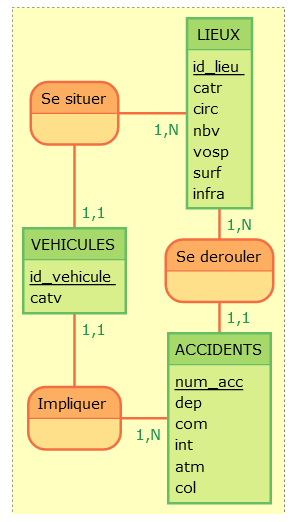
\includegraphics[width=8cm,height=8cm]{Images/MCD.png}
\caption{MCD}\label{mcd}
}
\end{figure}

\justify

\bigskip

\hypertarget{moduxe8le-organisationnel-de-donnuxe9es}{%
\section{Modèle Organisationnel de
données}\label{moduxe8le-organisationnel-de-donnuxe9es}}

\medskip

La version manuscrite du MOD ci dessous :

\textbf{LIEUX} (id\_lieu, num\_acc, catr, circ, nbv, vosp, surf,
infra)\\
\textbf{VEHICULES} (id\_vehicule, num\_acc, id\_lieu, catv)\\
\textbf{ACCIDENTS} (num\_acc, id\_lieu, dep, com, int, atm, col)

\medskip

À partir du Modèle Conceptuel des Données, nous avons créé le Modèle
Organisationnel des données, grâce à l'outil Concepteur de MAMP -
PhpMyAdmin:\\
\medskip

\begin{figure}
\hypertarget{mod}{%
\centering
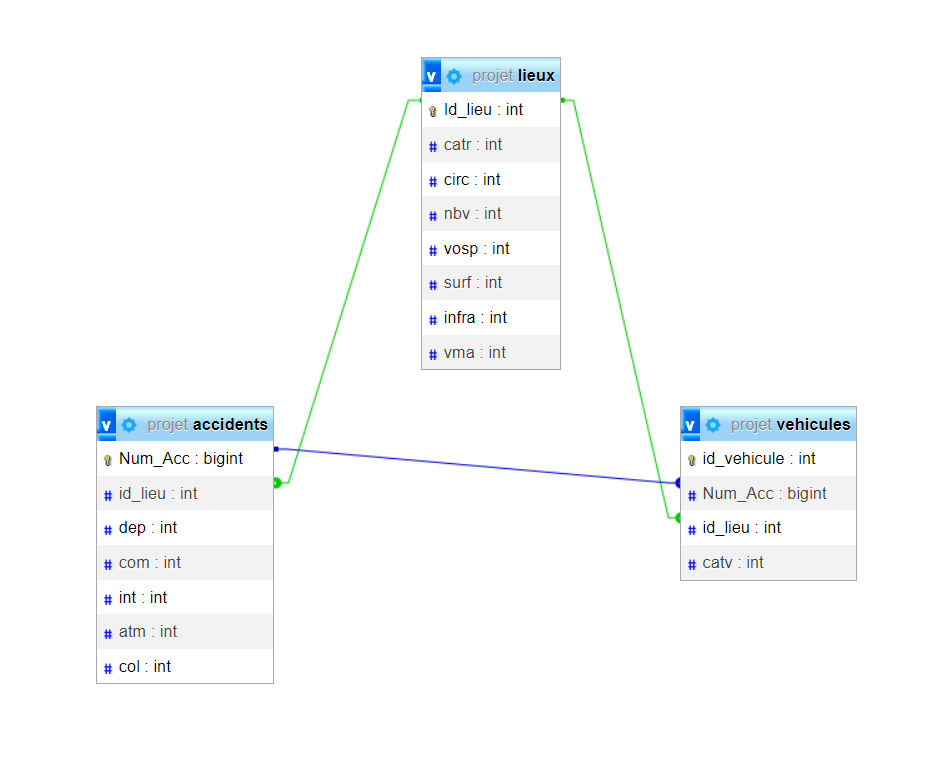
\includegraphics[width=8cm,height=8cm]{Images/MOD.png}
\caption{mod}\label{mod}
}
\end{figure}

\medskip

\hypertarget{pruxe9traitements}{%
\chapter{Prétraitements}\label{pruxe9traitements}}

\bigskip

Afin de manipuler aisaiment les données dans SQL, nous les avons fait
liés via les clés primaires et étrangères cités auparavant. Ensuite,
pour faciliter l'import de nos données sur la plateforme en ligne
{[}\url{https://filess.io/}{]}, nous avons dû modifier les tables dans
les différents classeurs Excel.

\medskip

-Pour la table \textbf{Accidents} : nous ne gardons pas les colonnes
décrivant le jour(jour), le mois(mois), l'heure à la minute près(hrmn),
la lumière au moment de l'accident(lum),l'année(an) car toutes les
données datent de la même année et l'adresse postale(adr) car la valeur
n'est pas renseignée pour tous les accidents donc moins pertinents.\\
\medskip

-Pour la table \textbf{Lieux} : Ont été exclus les colonnes décrivant
l'inclinaison de la route(prof), la largeur de la chaussée affectée à la
circulation hors bandes d'arrêt d'urgences et places de stationnement
ainsi que terre-plein-central (larrout), le numéro de la route(voie),
l'indice numérique de route(V1), la lettre indice alphanumérique de la
route(V2), le numéro du PR de rattachement(pr), la distance en mètres au
PR(pr1), le tracé en plan(plan) ainsi que la largeur du terre-plein
central(TPC) car cela ne nous semblaient pas être des variables
primordiales influençant énormément sur les chances d'être impliqués
dans un accident.\\
\medskip

-Pour la table \textbf{Vehicules} : Nous avons exclus les colonnes
décrivant le point de choc initial car ces dernières n'avaient
absolument aucun impact sur les chances d'être impliqués dans un
accident(choc), le type de motorisation du véhicule (motor) et le nombre
de personne dans le véhicule (occutc),le sens de circulation (senc),
l'obstacle fixe heurté si c'est le cas (obs), l'obstacle mobile heurté
si c'est le cas (obsm) ainsi que la manoeuvre effectué avant
l'accident(manv).

\hypertarget{requuxeates-ruxe9alisuxe9es}{%
\chapter{Requêtes réalisées}\label{requuxeates-ruxe9alisuxe9es}}

\scriptsize

\begin{Shaded}
\begin{Highlighting}[]
\CommentTok{\# install.packages("RMySQL")}
\CommentTok{\# install.packages("DBI")}
\FunctionTok{library}\NormalTok{(DBI)}
\end{Highlighting}
\end{Shaded}

\begin{verbatim}
## Warning: le package 'DBI' a été compilé avec la version R 4.2.3
\end{verbatim}

\begin{Shaded}
\begin{Highlighting}[]
\NormalTok{con }\OtherTok{\textless{}{-}}\NormalTok{ DBI}\SpecialCharTok{::}\FunctionTok{dbConnect}\NormalTok{(}
  \AttributeTok{drv =}\NormalTok{ RMySQL}\SpecialCharTok{::}\FunctionTok{MySQL}\NormalTok{(),    }
  \AttributeTok{host =} \StringTok{"nkv.h.filess.io"}\NormalTok{, }
  \AttributeTok{port =} \DecValTok{3307}\NormalTok{,               }
  \AttributeTok{username =} \StringTok{"Projet\_produceegg"}\NormalTok{, }
  \AttributeTok{password =} \StringTok{"5de5b1c29e6b2612ba58fcede731030b73ca5cf8"}\NormalTok{, }
  \AttributeTok{dbname =} \StringTok{"Projet\_produceegg"}    
\NormalTok{)}
\end{Highlighting}
\end{Shaded}

\begin{Shaded}
\begin{Highlighting}[]

\NormalTok{show }\KeywordTok{tables}\NormalTok{;}
\end{Highlighting}
\end{Shaded}

\begin{longtable}[]{@{}l@{}}
\caption{3 records}\tabularnewline
\toprule()
Tables\_in\_Projet\_produceegg \\
\midrule()
\endfirsthead
\toprule()
Tables\_in\_Projet\_produceegg \\
\midrule()
\endhead
accidents \\
lieux \\
vehicules \\
\bottomrule()
\end{longtable}

\medskip
\normalsize

\textbf{Requête 1:} \emph{Lister le nombre d'accidents par
département.}\\
Le département 75, celui de \emph{Paris} cumule le plus d'accidents.
Nous avons décidé d'ajouter la ligne ``having nombre \textgreater=1000''
par soucis d'affichage et ainsi on obtient \emph{le Graphe1} qui est un
peu trop surchargé mais on y voit clairement les départements les plus
impliqués dans des accidents. \medskip

\begin{Shaded}
\begin{Highlighting}[]
\KeywordTok{SELECT}\NormalTok{ dep, }\FunctionTok{COUNT}\NormalTok{(}\KeywordTok{DISTINCT}\NormalTok{ accidents.Num\_Acc) }\KeywordTok{as}\NormalTok{ nombre}
\KeywordTok{FROM}\NormalTok{ accidents }
\KeywordTok{GROUP} \KeywordTok{BY}\NormalTok{ dep}
\KeywordTok{HAVING}\NormalTok{ nombre }\OperatorTok{\textgreater{}=}\DecValTok{1000}
\KeywordTok{ORDER} \KeywordTok{BY}\NormalTok{ nombre }\KeywordTok{DESC}
\end{Highlighting}
\end{Shaded}

\begin{longtable}[]{@{}rr@{}}
\caption{6 records}\tabularnewline
\toprule()
dep & nombre \\
\midrule()
\endfirsthead
\toprule()
dep & nombre \\
\midrule()
\endhead
75 & 2133 \\
93 & 1240 \\
13 & 1175 \\
94 & 1095 \\
92 & 1081 \\
69 & 1062 \\
\bottomrule()
\end{longtable}

\medskip

\textbf{Requête 2:} \emph{Quelles sont les catégories de véhicule les
impliquées dans les accidents?}\\
La catégorie de véhicules la plus impliquée est la \emph{n°7} qui
correspond au \textbf{Véhicule Léger}.

\begin{Shaded}
\begin{Highlighting}[]
\KeywordTok{SELECT}\NormalTok{ vehicules.catv, }\FunctionTok{COUNT}\NormalTok{(}\KeywordTok{DISTINCT}\NormalTok{ accidents.Num\_Acc) }\KeywordTok{as}\NormalTok{ accident}
\KeywordTok{FROM}\NormalTok{ vehicules,accidents,lieux}
\KeywordTok{WHERE}\NormalTok{ accidents.id\_lieu}\OperatorTok{=}\NormalTok{lieux.Id\_lieu}
\KeywordTok{AND}\NormalTok{ vehicules.Num\_Acc}\OperatorTok{=}\NormalTok{accidents.Num\_Acc}
\KeywordTok{GROUP} \KeywordTok{BY}\NormalTok{ vehicules.catv}
\KeywordTok{ORDER} \KeywordTok{BY}\NormalTok{ accident }\KeywordTok{DESC}\NormalTok{;}
\end{Highlighting}
\end{Shaded}

\begin{longtable}[]{@{}rr@{}}
\caption{Displaying records 1 - 10}\tabularnewline
\toprule()
catv & accident \\
\midrule()
\endfirsthead
\toprule()
catv & accident \\
\midrule()
\endhead
7 & 19191 \\
33 & 3098 \\
10 & 2822 \\
1 & 2163 \\
2 & 1592 \\
30 & 1393 \\
32 & 967 \\
50 & 752 \\
31 & 699 \\
15 & 415 \\
\bottomrule()
\end{longtable}

\medskip

\textbf{Requête 3:} \emph{Quels sont les types de collisions les plus
fréquents lors des accidents }?\\
Les collisions impliquants \emph{deux voitures par le coté} sont les
plus fréquentes lors des accidents.

\begin{Shaded}
\begin{Highlighting}[]
\KeywordTok{SELECT}\NormalTok{ col, }\FunctionTok{COUNT}\NormalTok{(}\OperatorTok{*}\NormalTok{)}
\KeywordTok{FROM}\NormalTok{ accidents}
\KeywordTok{GROUP} \KeywordTok{BY}\NormalTok{ col}
\KeywordTok{ORDER} \KeywordTok{BY} \FunctionTok{COUNT}\NormalTok{(}\OperatorTok{*}\NormalTok{) }\KeywordTok{DESC}
\end{Highlighting}
\end{Shaded}

\begin{longtable}[]{@{}rr@{}}
\caption{8 records}\tabularnewline
\toprule()
col & COUNT(*) \\
\midrule()
\endfirsthead
\toprule()
col & COUNT(*) \\
\midrule()
\endhead
3 & 7779 \\
6 & 7219 \\
2 & 3388 \\
1 & 2646 \\
7 & 2306 \\
4 & 932 \\
5 & 725 \\
-1 & 5 \\
\bottomrule()
\end{longtable}

\textbf{Requête 4:} \emph{Quels sont les infrastructures/aménagements
les plus touchés par les accidents?}\\
Dans plus de la moitié des accidents aucune infrastructure n'est touché.

\begin{Shaded}
\begin{Highlighting}[]
\KeywordTok{SELECT}\NormalTok{ lieux.infra, }\FunctionTok{COUNT}\NormalTok{(}\KeywordTok{DISTINCT}\NormalTok{ accidents.Num\_Acc) }\KeywordTok{as} \FunctionTok{count} 
\KeywordTok{FROM}\NormalTok{ accidents,lieux}
\KeywordTok{WHERE}\NormalTok{ accidents.id\_lieu}\OperatorTok{=}\NormalTok{lieux.id\_lieu}
\KeywordTok{GROUP} \KeywordTok{by}\NormalTok{ lieux.infra}
\KeywordTok{ORDER} \KeywordTok{BY} \FunctionTok{count} \KeywordTok{DESC}
\end{Highlighting}
\end{Shaded}

\begin{longtable}[]{@{}rr@{}}
\caption{Displaying records 1 - 10}\tabularnewline
\toprule()
infra & count \\
\midrule()
\endfirsthead
\toprule()
infra & count \\
\midrule()
\endhead
0 & 21025 \\
5 & 1253 \\
9 & 904 \\
2 & 373 \\
3 & 368 \\
1 & 310 \\
6 & 249 \\
-1 & 247 \\
8 & 161 \\
4 & 98 \\
\bottomrule()
\end{longtable}

\medskip

\textbf{Requête 5:} \emph{Quels états de la surface de la route sont les
plus dangereux?}\\
Quasiment tous les accidents ont lieu quand sur des surfaces de
\emph{routes normales} suivis de près par les accidents sur des surfaces
\emph{mouillées}.

\begin{Shaded}
\begin{Highlighting}[]
\KeywordTok{SELECT}\NormalTok{ lieux.surf, }\FunctionTok{COUNT}\NormalTok{(}\KeywordTok{DISTINCT}\NormalTok{ accidents.Num\_Acc) }
\KeywordTok{FROM}\NormalTok{ accidents,lieux }
\KeywordTok{WHERE}\NormalTok{ accidents.id\_lieu}\OperatorTok{=}\NormalTok{lieux.Id\_lieu }
\KeywordTok{GROUP} \KeywordTok{BY}\NormalTok{ lieux.surf }
\KeywordTok{ORDER} \KeywordTok{BY}\NormalTok{ \textasciigrave{}COUNT(}\KeywordTok{DISTINCT}\NormalTok{ accidents.Num\_Acc)\textasciigrave{} }\KeywordTok{DESC}
\end{Highlighting}
\end{Shaded}

\begin{longtable}[]{@{}rr@{}}
\caption{Displaying records 1 - 10}\tabularnewline
\toprule()
surf & COUNT(DISTINCT accidents.Num\_Acc) \\
\midrule()
\endfirsthead
\toprule()
surf & COUNT(DISTINCT accidents.Num\_Acc) \\
\midrule()
\endhead
1 & 19758 \\
2 & 4826 \\
9 & 155 \\
7 & 117 \\
3 & 39 \\
6 & 33 \\
8 & 30 \\
5 & 26 \\
-1 & 10 \\
4 & 6 \\
\bottomrule()
\end{longtable}

\medskip

\textbf{Requête 6:} \emph{Sous quelles vitessses maximales autorisées
(vma) sur les routes sont répertoriées les accidents les plus à
risques.}\\
Les accidents ont plutôt tendance à avoir lieu sur des voix à \emph{50
Km/h}.

\begin{Shaded}
\begin{Highlighting}[]
\KeywordTok{SELECT}\NormalTok{ lieux.vma, }\FunctionTok{COUNT}\NormalTok{(}\KeywordTok{DISTINCT}\NormalTok{ accidents.Num\_Acc) }
\KeywordTok{FROM}\NormalTok{ accidents,lieux }
\KeywordTok{WHERE}\NormalTok{ accidents.id\_lieu}\OperatorTok{=}\NormalTok{lieux.Id\_lieu }
\KeywordTok{GROUP} \KeywordTok{BY}\NormalTok{ lieux.vma }
\KeywordTok{ORDER} \KeywordTok{BY}\NormalTok{ \textasciigrave{}COUNT(}\KeywordTok{DISTINCT}\NormalTok{ accidents.Num\_Acc)\textasciigrave{} }\KeywordTok{DESC}
\end{Highlighting}
\end{Shaded}

\begin{longtable}[]{@{}rr@{}}
\caption{Displaying records 1 - 10}\tabularnewline
\toprule()
vma & COUNT(DISTINCT accidents.Num\_Acc) \\
\midrule()
\endfirsthead
\toprule()
vma & COUNT(DISTINCT accidents.Num\_Acc) \\
\midrule()
\endhead
50 & 12330 \\
30 & 3454 \\
80 & 3362 \\
90 & 2021 \\
70 & 1810 \\
110 & 907 \\
130 & 470 \\
-1 & 414 \\
20 & 61 \\
10 & 47 \\
\bottomrule()
\end{longtable}

\medskip

\textbf{Requête 7:} \emph{Lister le nombre de voies(nbv) selon les
accidents les plus fréquents .}\\
Ces accidents sont répertoriés le plus souvent sur les routes à \emph{2
voies.}

\begin{Shaded}
\begin{Highlighting}[]
\KeywordTok{SELECT}\NormalTok{ lieux.nbv, }\FunctionTok{COUNT}\NormalTok{(}\KeywordTok{DISTINCT}\NormalTok{ accidents.Num\_Acc) }
\KeywordTok{FROM}\NormalTok{ accidents,lieux }
\KeywordTok{WHERE}\NormalTok{ accidents.id\_lieu}\OperatorTok{=}\NormalTok{lieux.Id\_lieu }
\KeywordTok{GROUP} \KeywordTok{BY}\NormalTok{ lieux.nbv }
\KeywordTok{ORDER} \KeywordTok{BY}\NormalTok{ \textasciigrave{}COUNT(}\KeywordTok{DISTINCT}\NormalTok{ accidents.Num\_Acc)\textasciigrave{} }\KeywordTok{DESC}\NormalTok{;}
\end{Highlighting}
\end{Shaded}

\begin{longtable}[]{@{}rr@{}}
\caption{Displaying records 1 - 10}\tabularnewline
\toprule()
nbv & COUNT(DISTINCT accidents.Num\_Acc) \\
\midrule()
\endfirsthead
\toprule()
nbv & COUNT(DISTINCT accidents.Num\_Acc) \\
\midrule()
\endhead
2 & 15162 \\
4 & 3024 \\
1 & 2667 \\
3 & 2010 \\
6 & 658 \\
0 & 547 \\
5 & 378 \\
-1 & 221 \\
8 & 208 \\
7 & 54 \\
\bottomrule()
\end{longtable}

\medskip

\textbf{Requête 8:} \emph{Quelles sont les conditions atmosphériques
(atm) ayant causées plus d'accidents?}\\
Quasiment tous les accidents ont lieu quand les conditions
atmosphériques sont \emph{1: normale} et \emph{2: mouillées}.

\begin{Shaded}
\begin{Highlighting}[]
\KeywordTok{SELECT}\NormalTok{ atm,}\FunctionTok{COUNT}\NormalTok{(}\KeywordTok{DISTINCT}\NormalTok{ accidents.Num\_Acc) }\KeywordTok{as}\NormalTok{ nombre}
\KeywordTok{FROM}\NormalTok{ accidents}
\KeywordTok{GROUP} \KeywordTok{BY}\NormalTok{ atm}
\KeywordTok{ORDER} \KeywordTok{BY}\NormalTok{ nombre }\KeywordTok{DESC}
\end{Highlighting}
\end{Shaded}

\begin{longtable}[]{@{}rr@{}}
\caption{Displaying records 1 - 10}\tabularnewline
\toprule()
atm & nombre \\
\midrule()
\endfirsthead
\toprule()
atm & nombre \\
\midrule()
\endhead
1 & 19588 \\
2 & 2782 \\
8 & 1074 \\
3 & 521 \\
7 & 447 \\
5 & 337 \\
9 & 143 \\
4 & 58 \\
6 & 43 \\
-1 & 7 \\
\bottomrule()
\end{longtable}

\bigskip

\hypertarget{moduxe9lisation-statistique}{%
\chapter{Modélisation statistique}\label{moduxe9lisation-statistique}}

Pour faciliter la manipulation des requêtes avec Rstudio, nous avons dû
ajuster l'écriture des requêtes qui restent dans le fond les mêmes avec
des résultats similaires.

\medskip

\textbf{Requête 1 \#Graphe1 :} \emph{Porte sur la fréquence des
accidents, requête 1 en SQL.}\\
On peut constater que le département ayant le plus d'accident est le
département de Paris et ceux d'après sont les départements autour de
Paris (93,94 et 92) à l'exception du 13 qui est les Bouches-du-Rhône où
se trouve Marseille. Ces résultats ne sont pas si surprenant car ce sont
sûrement les départements où il y a le plus de circulation.

\medskip

\textbf{Requête 2 \#Graphe2 :} \emph{Porte sur les catégories de
véhicules} impliquées dans les accidents, requête 2 en SQL.\\
La requête nous a permis de voir que les catégories de véhicules les
plus impliquées dans les accidents sont les véhicules de type 7 et 33
selon les résultats de notre requête sql. Les véhicules de type 7 sont
des véhicules légers, et donc regroupe tous les véhicules de moins de
3,5 tonnes(les voitures) et les véhicules de type 33 sont les
motocyclettes.\\
Les motocyclettes et les voitures légers selon le camembert obtenu à
partir de la requête faite sur R sont les véhicules qui enregistre le
plus grand nombre d'accidents; ce qui est logique car se sont les
véhicules les plus utilisés sur la route.

\medskip

\textbf{Requête 3 \#Graphe3 :} \emph{Porte sur les collisions, requête 3
en sql.}\\
Nous avons fait une requête afin d'analyser les types de collisions les
plus fréquents dans les départements les plus à risques. Cette requête
sql nous a donné des résultats selon les 8 types de collisions . Mais
nous nous intéressons aux deux types de collisions qui regroupent le
plus grand nombre d'accidents. Nous voyons que les collisions de types 3
et 6 sont les plus fréquentes. Le type 3 désigne la collision de deux
véhicules par le côté et le type 6 désigne toutes les collisions simples
qui n'inclue qu'un seul véhicule.\\
Nous avons comparé les résultats des types collisions les plus fréquents
dans tous les départements aux résultats des types de collisions les
plus fréquents dans les régions les plus à risques et avons bien
remarqué sur les camemberts qu'ils sont similaires. La seule différence
notable est que les collisions de type 3 sont un peu plus forte dans les
départements les plus risques.

\medskip

\textbf{Requête 4 \#Graphe4 :} \emph{Porte sur les surfaces, requête 5
en sql.}\\
En outre, nous avons fait cette requête afin de connaître les états de
la route les plus dangereuses. Selon les résultats de notre requête sql
se sont les états de surface de la route de type 1 et 2 qui causent le
plus d'accidents. Celui de type 1 représente lorsque la route a un état
normal, c'est à dire que le sol n'est ni enneigé ou mouillé, il y a rien
sur la route. L'état de surface de type 2, c'est lorsque le sol est
mouillé. Nous remarquons qu'en situation de surface normale, il y'a
beaucoup plus d'accidents que la surface des routes est mouillée,
lorsqu'il pleut. Cependant, nous aurons tendance à penser que c'est
l'inverse qui se produit mais ce n'est pas le cas en réalité. C'est
certainement dû au fait qu'il y a plus de circulation lorsque le sol
n'est pas mouillée que lorsqu'il l'est.

\medskip

\textbf{Requête 5 \#Graphe5 :} \emph{Porte sur la vitesse maximale,
requête 6 en sql.}

On constate que dans la plupart des accidents la vitesse maximale
autorisée est de 50 km/h. On peut voir que c'est peu près la moitié des
accidents qui sont concernés et qui se produisent donc très certainement
en agglomération. Et juste en dessous la seconde vitesse maximale
autorisée impliquée dans le plus d'accident est 30 km /h. Ainsi, on peut
en déduire que la majorité des accidents se produisent en agglomération
ce qui n'est pas très étonnant car il est plus compliqué de rouler en
agglomération que sur la route hors agglomération. On peut voir qu'un
bon quart des accidents on l'air de se dérouler sur des départementales
et le reste probablement sur l'autoroute.

\medskip

\textbf{Requête 6 \#Graphe6 :} \emph{Porte sur les conditions
atmosphériques les plus fréquentes,requête 8 en sql.}\\
On remarque assez facilement que la grande majorité des accidents ont
lieu pour la condition atmosphérique 1 qui correspond à des conditions
atmosphériques normales. On peut donc en conclure que ces dernières ont
peu d'impact sur les accidents. On remarque tout de même que les
conditions atmosphériques 2 et 8, qui correspondent respectivement à de
la pluie légère et à un temps couvert se démarquent un peu mais cela
peut s'expliquer par le fait qu'il va certainement avoir plus de gens
qui roulent lorsqu'il pleut ou qu'il fait couvert que lorsqu'il neige ou
qu'il y a une tempête.

\hypertarget{difficultuxe9s-et-conclusion}{%
\chapter{Difficultés et Conclusion}\label{difficultuxe9s-et-conclusion}}

\hypertarget{difficultuxe9s}{%
\section{Difficultés}\label{difficultuxe9s}}

\medskip

Au cours de la réalisation de ce projet, nous avons rencontré certes peu
de difficulté mais les quelques difficultés que nous avons pu rencontrer
nous ont donné du fil à retordre.\\
La principale difficulté, qui est aussi la seule notable, que nous avons
rencontrés a été la mise en ligne de notre base de données, pour faire
ceci il fallait que notre base de données ait une taille inférieure à 10
Mb et à chaque fois que nous importions une base de données en ligne
elle était acceptée pour ensuite être désactivé quelques jours plus
tard. La raison était que la vraie taille de la base de données mise en
ligne mettait plusieurs jours à être calculé et ne correspondais pas
exactement à la taille qu'on avait. Nous avons finalement réussi à la
mettre en ligne après l'avoir filtré plusieurs fois.\\
Nous avons aussi rencontré une légère difficulté sur R pour faire les
graphiques car juste recopier les requêtes SQL ne fonctionner pas, il a
fallu les modifier pour pouvoir faire les graphiques que l'on voulait.

\bigskip

\hypertarget{conclusion}{%
\section{Conclusion}\label{conclusion}}

\medskip

On remarque que les conditions les plus à risques ne sont pas vraiment
celles impliqués le plus dans les accidents et qu'au contraire ce sont
pour les conditions les moins à risque qu'il y a le plus d'accident.
Cela s'explique par le fait qu'il doit simplement y avoir plus de gens
qui roule lorsque les conditions sont moins à risque ce qui fait qu'en
fin de compte ce n'est pas forcément moins dangereux car comme il y a
plus de monde qui en circulation, il y a plus de chance d'être impliqué
dans un accident.

\hypertarget{annexes}{%
\chapter*{Annexes}\label{annexes}}
\addcontentsline{toc}{chapter}{Annexes}

\hypertarget{graphiques-concernant-la-moduxe9lisation-en-r}{%
\section*{Graphiques concernant la modélisation en
R}\label{graphiques-concernant-la-moduxe9lisation-en-r}}
\addcontentsline{toc}{section}{Graphiques concernant la modélisation en
R}

\medskip

\textbf{Graphe 1}

\begin{Shaded}
\begin{Highlighting}[]
\NormalTok{Z}\OtherTok{\textless{}{-}}\FunctionTok{dbGetQuery}\NormalTok{(con,}\StringTok{"SELECT accidents.dep}
\StringTok{FROM accidents,lieux}
\StringTok{WHERE accidents.id\_lieu=lieux.Id\_lieu;"}\NormalTok{)}
\FunctionTok{pie}\NormalTok{(}\FunctionTok{table}\NormalTok{(Z), }\AttributeTok{col =} \FunctionTok{rainbow}\NormalTok{(}\DecValTok{50}\NormalTok{))}
\end{Highlighting}
\end{Shaded}

\includegraphics{rapport-G04_files/figure-latex/unnamed-chunk-11-1.pdf}

\medskip

\textbf{Graphe 2}

\begin{Shaded}
\begin{Highlighting}[]
\NormalTok{Z}\OtherTok{\textless{}{-}}\FunctionTok{dbGetQuery}\NormalTok{(con,}\StringTok{"SELECT vehicules.catv}
\StringTok{FROM vehicules,accidents,lieux}
\StringTok{WHERE accidents.id\_lieu=lieux.Id\_lieu AND vehicules.Num\_Acc=accidents.Num\_Acc }
\StringTok{"}\NormalTok{)}
\FunctionTok{pie}\NormalTok{(}\FunctionTok{table}\NormalTok{(Z), }\AttributeTok{col =} \FunctionTok{c}\NormalTok{(}\StringTok{"gray"}\NormalTok{, }\StringTok{"red"}\NormalTok{,}\StringTok{"yellow"}\NormalTok{,}\StringTok{"blue"}\NormalTok{,}\StringTok{"pink"}\NormalTok{,}\StringTok{"purple"}
\NormalTok{                      ,}\StringTok{"green"}\NormalTok{,}\StringTok{"brown"}\NormalTok{,}\StringTok{"white"}\NormalTok{,}\StringTok{"orange"}\NormalTok{))}
\end{Highlighting}
\end{Shaded}

\includegraphics{rapport-G04_files/figure-latex/unnamed-chunk-12-1.pdf}

\medskip

\textbf{Grape 3}

\begin{Shaded}
\begin{Highlighting}[]
\NormalTok{Z}\OtherTok{\textless{}{-}}\FunctionTok{dbGetQuery}\NormalTok{(con,}\StringTok{"SELECT col}
\StringTok{FROM accidents"}\NormalTok{)}
\FunctionTok{pie}\NormalTok{(}\FunctionTok{table}\NormalTok{(Z), }\AttributeTok{col =} \FunctionTok{c}\NormalTok{(}\StringTok{"red"}\NormalTok{,}\StringTok{"orange"}\NormalTok{,}\StringTok{"pink"}\NormalTok{, }\StringTok{"yellow"}\NormalTok{,}\StringTok{"purple"}\NormalTok{,}
                      \StringTok{"green"}\NormalTok{,}\StringTok{"blue"}\NormalTok{, }\StringTok{"darkblue"}\NormalTok{))}
\end{Highlighting}
\end{Shaded}

\includegraphics{rapport-G04_files/figure-latex/unnamed-chunk-13-1.pdf}

\begin{Shaded}
\begin{Highlighting}[]
\CommentTok{\#graphe de la répartition du type de collisions dans les départements }
\CommentTok{\#les plus à risques}
\NormalTok{Z}\OtherTok{\textless{}{-}}\FunctionTok{dbGetQuery}\NormalTok{(con,}\StringTok{"SELECT col}
\StringTok{FROM accidents}
\StringTok{where dep=13 OR dep=94 OR dep=93 OR dep=92 OR dep=75 OR dep=69}
\StringTok{"}\NormalTok{)}
\FunctionTok{pie}\NormalTok{(}\FunctionTok{table}\NormalTok{(Z), }\AttributeTok{col =} \FunctionTok{c}\NormalTok{(}\StringTok{"red"}\NormalTok{,}\StringTok{"orange"}\NormalTok{,}\StringTok{"pink"}\NormalTok{, }\StringTok{"yellow"}\NormalTok{,}\StringTok{"purple"}\NormalTok{,}
                      \StringTok{"green"}\NormalTok{,}\StringTok{"blue"}\NormalTok{, }\StringTok{"darkblue"}\NormalTok{))}
\end{Highlighting}
\end{Shaded}

\includegraphics{rapport-G04_files/figure-latex/unnamed-chunk-14-1.pdf}

\medskip

\textbf{Graphe 4}:

\begin{Shaded}
\begin{Highlighting}[]
\NormalTok{Z}\OtherTok{\textless{}{-}}\FunctionTok{dbGetQuery}\NormalTok{(con,}\StringTok{"SELECT lieux.surf FROM accidents,}
\StringTok{              lieux WHERE accidents.id\_lieu=lieux.Id\_lieu"}\NormalTok{)}
\FunctionTok{barplot}\NormalTok{(}\FunctionTok{table}\NormalTok{(Z), }\AttributeTok{col =} \FunctionTok{c}\NormalTok{(}\StringTok{"red"}\NormalTok{,}\StringTok{"orange"}\NormalTok{,}\StringTok{"pink"}\NormalTok{, }\StringTok{"yellow"}\NormalTok{,}
                          \StringTok{"purple"}\NormalTok{, }\StringTok{"green"}\NormalTok{,}\StringTok{"blue"}\NormalTok{, }\StringTok{"darkblue"}\NormalTok{,}\StringTok{"gray"}\NormalTok{,}\StringTok{"black"}\NormalTok{))}
\end{Highlighting}
\end{Shaded}

\includegraphics{rapport-G04_files/figure-latex/unnamed-chunk-15-1.pdf}

\medskip

\textbf{Graphe 5 }

\begin{Shaded}
\begin{Highlighting}[]
\NormalTok{Z}\OtherTok{\textless{}{-}}\FunctionTok{dbGetQuery}\NormalTok{(con,}\StringTok{"SELECT lieux.vma FROM accidents,}
\StringTok{lieux WHERE accidents.id\_lieu=lieux.Id\_lieu }
\StringTok{"}\NormalTok{)}
\FunctionTok{pie}\NormalTok{(}\FunctionTok{table}\NormalTok{(Z), }\AttributeTok{col =} \FunctionTok{c}\NormalTok{(}\StringTok{"red"}\NormalTok{,}\StringTok{"orange"}\NormalTok{,}\StringTok{"pink"}\NormalTok{, }\StringTok{"yellow"}\NormalTok{,}\StringTok{"purple"}\NormalTok{,}
                      \StringTok{"green"}\NormalTok{,}\StringTok{"blue"}\NormalTok{, }\StringTok{"darkblue"}\NormalTok{,}\StringTok{"gray"}\NormalTok{,}\StringTok{"black"}\NormalTok{))}
\end{Highlighting}
\end{Shaded}

\includegraphics{rapport-G04_files/figure-latex/unnamed-chunk-16-1.pdf}

\medskip

\textbf{Graphe 6 }

\begin{Shaded}
\begin{Highlighting}[]
\NormalTok{Z}\OtherTok{\textless{}{-}}\FunctionTok{dbGetQuery}\NormalTok{(con,}\StringTok{"SELECT atm}
\StringTok{FROM accidents"}\NormalTok{)}
\FunctionTok{barplot}\NormalTok{(}\FunctionTok{table}\NormalTok{(Z), }\AttributeTok{col =} \FunctionTok{c}\NormalTok{(}\StringTok{"blue"}\NormalTok{,}\StringTok{"orange"}\NormalTok{,}\StringTok{"pink"}\NormalTok{, }\StringTok{"yellow"}\NormalTok{,}\StringTok{"purple"}\NormalTok{, }\StringTok{"green"}\NormalTok{,}
                          \StringTok{"blue"}\NormalTok{, }\StringTok{"darkblue"}\NormalTok{,}\StringTok{"gray"}\NormalTok{,}\StringTok{"black"}\NormalTok{))}
\end{Highlighting}
\end{Shaded}

\includegraphics{rapport-G04_files/figure-latex/unnamed-chunk-17-1.pdf}

\medskip

\textbf{Graphe 7 }

\begin{Shaded}
\begin{Highlighting}[]
\NormalTok{Z}\OtherTok{\textless{}{-}}\FunctionTok{dbGetQuery}\NormalTok{(con,}\StringTok{"SELECT lieux.nbv FROM accidents,}
\StringTok{lieux WHERE accidents.id\_lieu=lieux.Id\_lieu ;}
\StringTok{"}\NormalTok{)}
\FunctionTok{barplot}\NormalTok{(}\FunctionTok{table}\NormalTok{(Z), }\AttributeTok{col =} \FunctionTok{c}\NormalTok{(}\StringTok{"red"}\NormalTok{,}\StringTok{"orange"}\NormalTok{,}\StringTok{"pink"}\NormalTok{, }\StringTok{"yellow"}\NormalTok{,}\StringTok{"purple"}\NormalTok{, }\StringTok{"green"}
\NormalTok{                        ,}\StringTok{"blue"}\NormalTok{, }\StringTok{"darkblue"}\NormalTok{,}\StringTok{"gray"}\NormalTok{,}\StringTok{"black"}\NormalTok{))}
\end{Highlighting}
\end{Shaded}

\includegraphics{rapport-G04_files/figure-latex/unnamed-chunk-18-1.pdf}

\begin{Shaded}
\begin{Highlighting}[]
\FunctionTok{dbDisconnect}\NormalTok{(con)}
\end{Highlighting}
\end{Shaded}

\begin{verbatim}
## [1] TRUE
\end{verbatim}







\end{document}

